\documentclass[final,t,unknownkeysallowed]{beamer}
\mode<presentation>
\usetheme{Purdue}
\usepackage{multirow}


\setbeamerfont{itemize}{size=\normalsize}
\setbeamerfont{itemize/enumerate body}{size=\normalsize}
\setbeamerfont{itemize/enumerate subbody}{size=\normalsize}

\usepackage{times}
\usepackage{amsmath,amsthm, amssymb, latexsym}
\usepackage{exscale}
%\boldmath
\usepackage{booktabs, array}
%\usepackage{rotating}
\newenvironment{lisp}{\begin{tt}\begin{tabular}[t]{l}}{\end{tabular}\end{tt}}
\usepackage[english]{babel}
\usepackage[latin1]{inputenc}
\usepackage[orientation=landscape,size=custom,width=135.46667,height=101.6,scale=1.5]{beamerposter}
\listfiles
\graphicspath{{figure/}}
% Display a grid to help align images
%\beamertemplategridbackground[1cm]

\title{\Huge Exploration of Hierarchical Softmax for Neural Language Models}
\author{Nan Jiang, Wenge Rong, Min Gao, Yikang Shen and Zhang Xiong}
\institute[School of ECE]{Beihang University, Chongqing University and Universite de Montreal }
\date[Aug. 25 , 2017]{Aug. 25 , 2017}

\usepackage{xspace}

\begin{document}
\begin{frame}{}
  \begin{columns}[t]
    \begin{column}{.3\linewidth}

      \begin{block}{Softmax with Over-large Vocabularies}
      \begin{figure}
      \centering{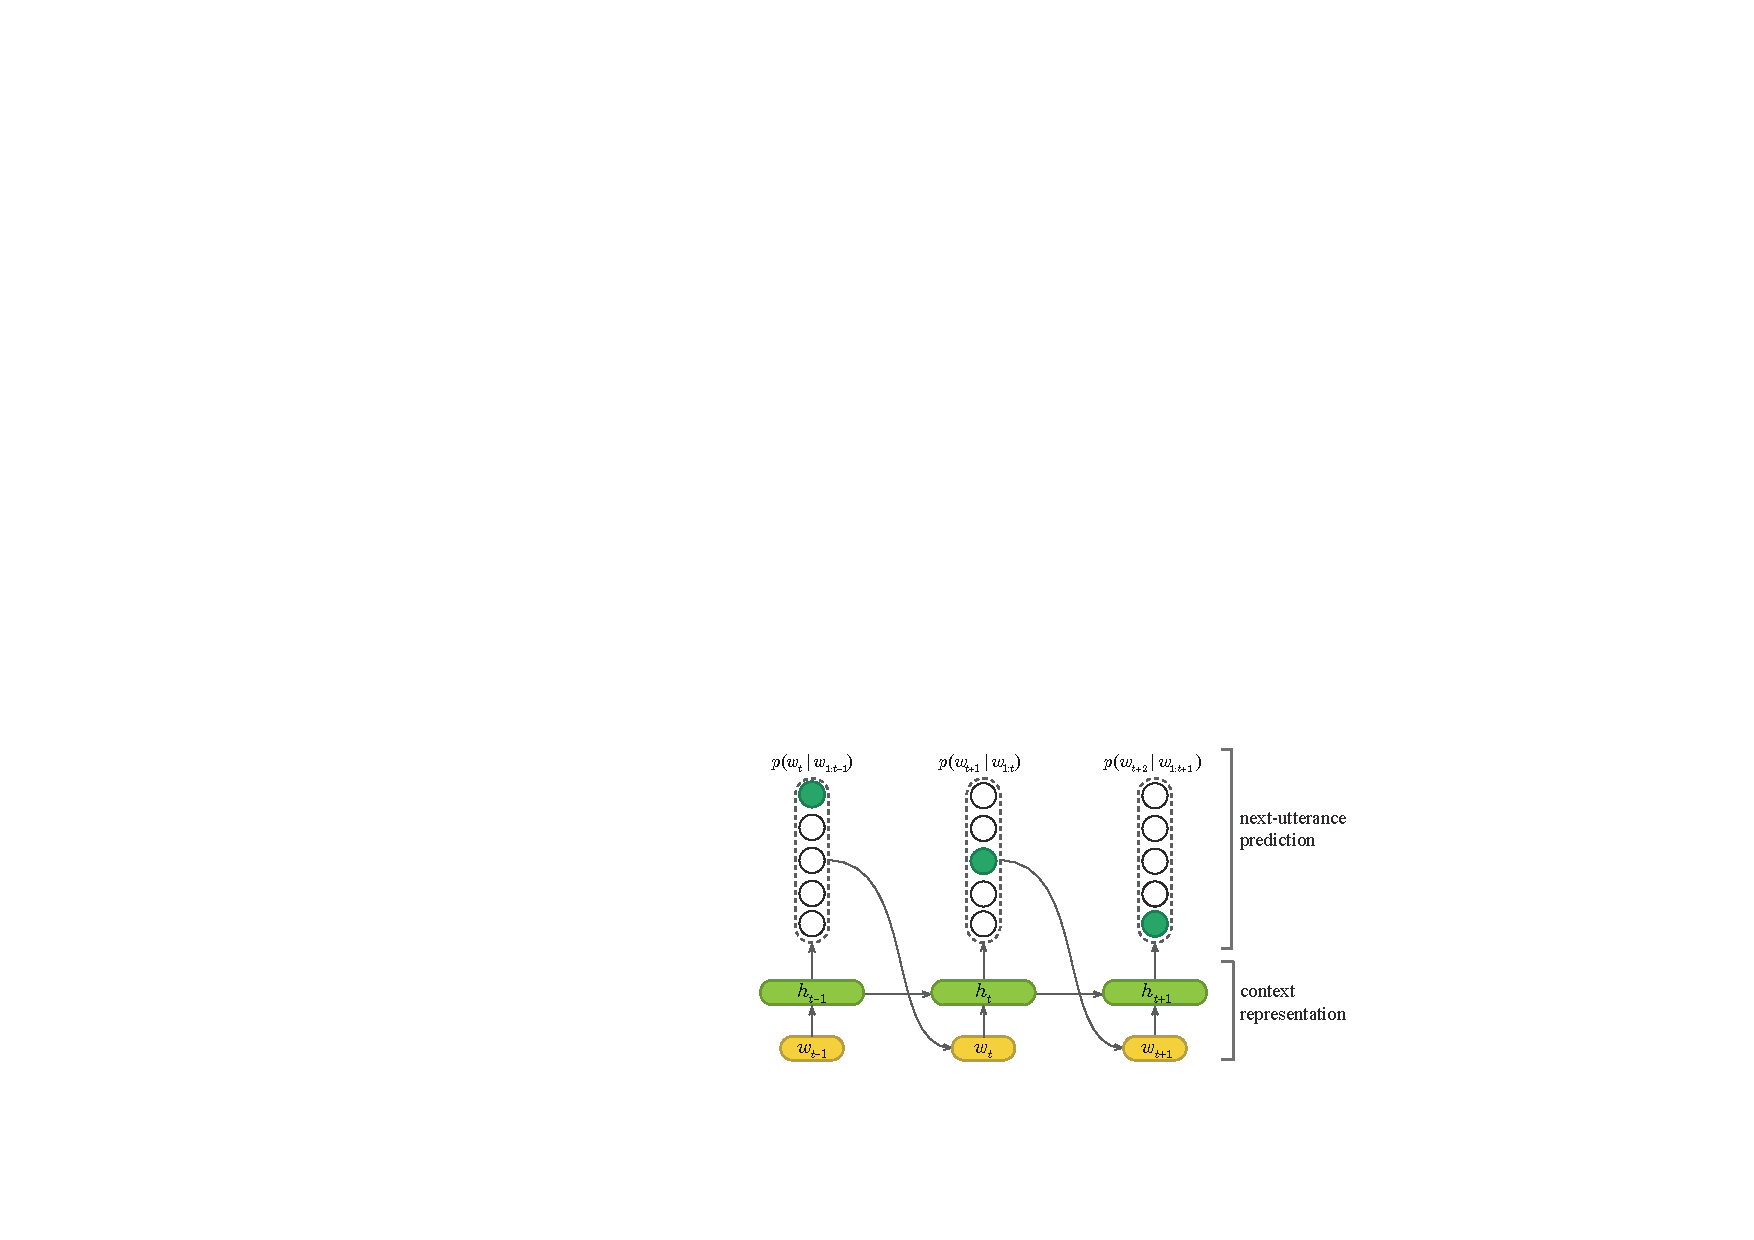
\includegraphics[width=0.7\linewidth]{lm}}
      \caption{Recurrent Neural Language Model.}
      \end{figure}
      \begin{equation}\small
         \log p(w_1,\cdots, w_T ) = \sum_{t=1}^T \log p(w_t | w_{1:t-1}),\quad p(w_i|h)=\frac{\exp(h^\top v_{w_i})}{\sum_{w_j\in \mathcal{V}}{\exp(h^\top v_{w_j} )}}
    \end{equation}
    \begin{itemize}
	\item \textbf{Vocabulary Truncation:}
    the vocabulary are split into a short-list of the most frequent words and a tail of OOV words.
	\item \textbf{Sampling based Approximation:}
    compute only a tiny fraction of the outputs dimensions to achieve computational efficiency, like Noise contrastive estimation, Importance sampling, Blackout sampling and etc.
	\item \textbf{Vocabulary Factorization:}
    decompose the flattened architecture of vocabulary into a class structure (i.e., class-based hierarchical softmax) or hierarchical binary tree (i.e., tree-based hierarchical softmax).
    \end{itemize}
      \end{block}
      
      
      \begin{block}{Parallelised Tree-based Hierarchical Softmax}
      \begin{figure}
      \centering{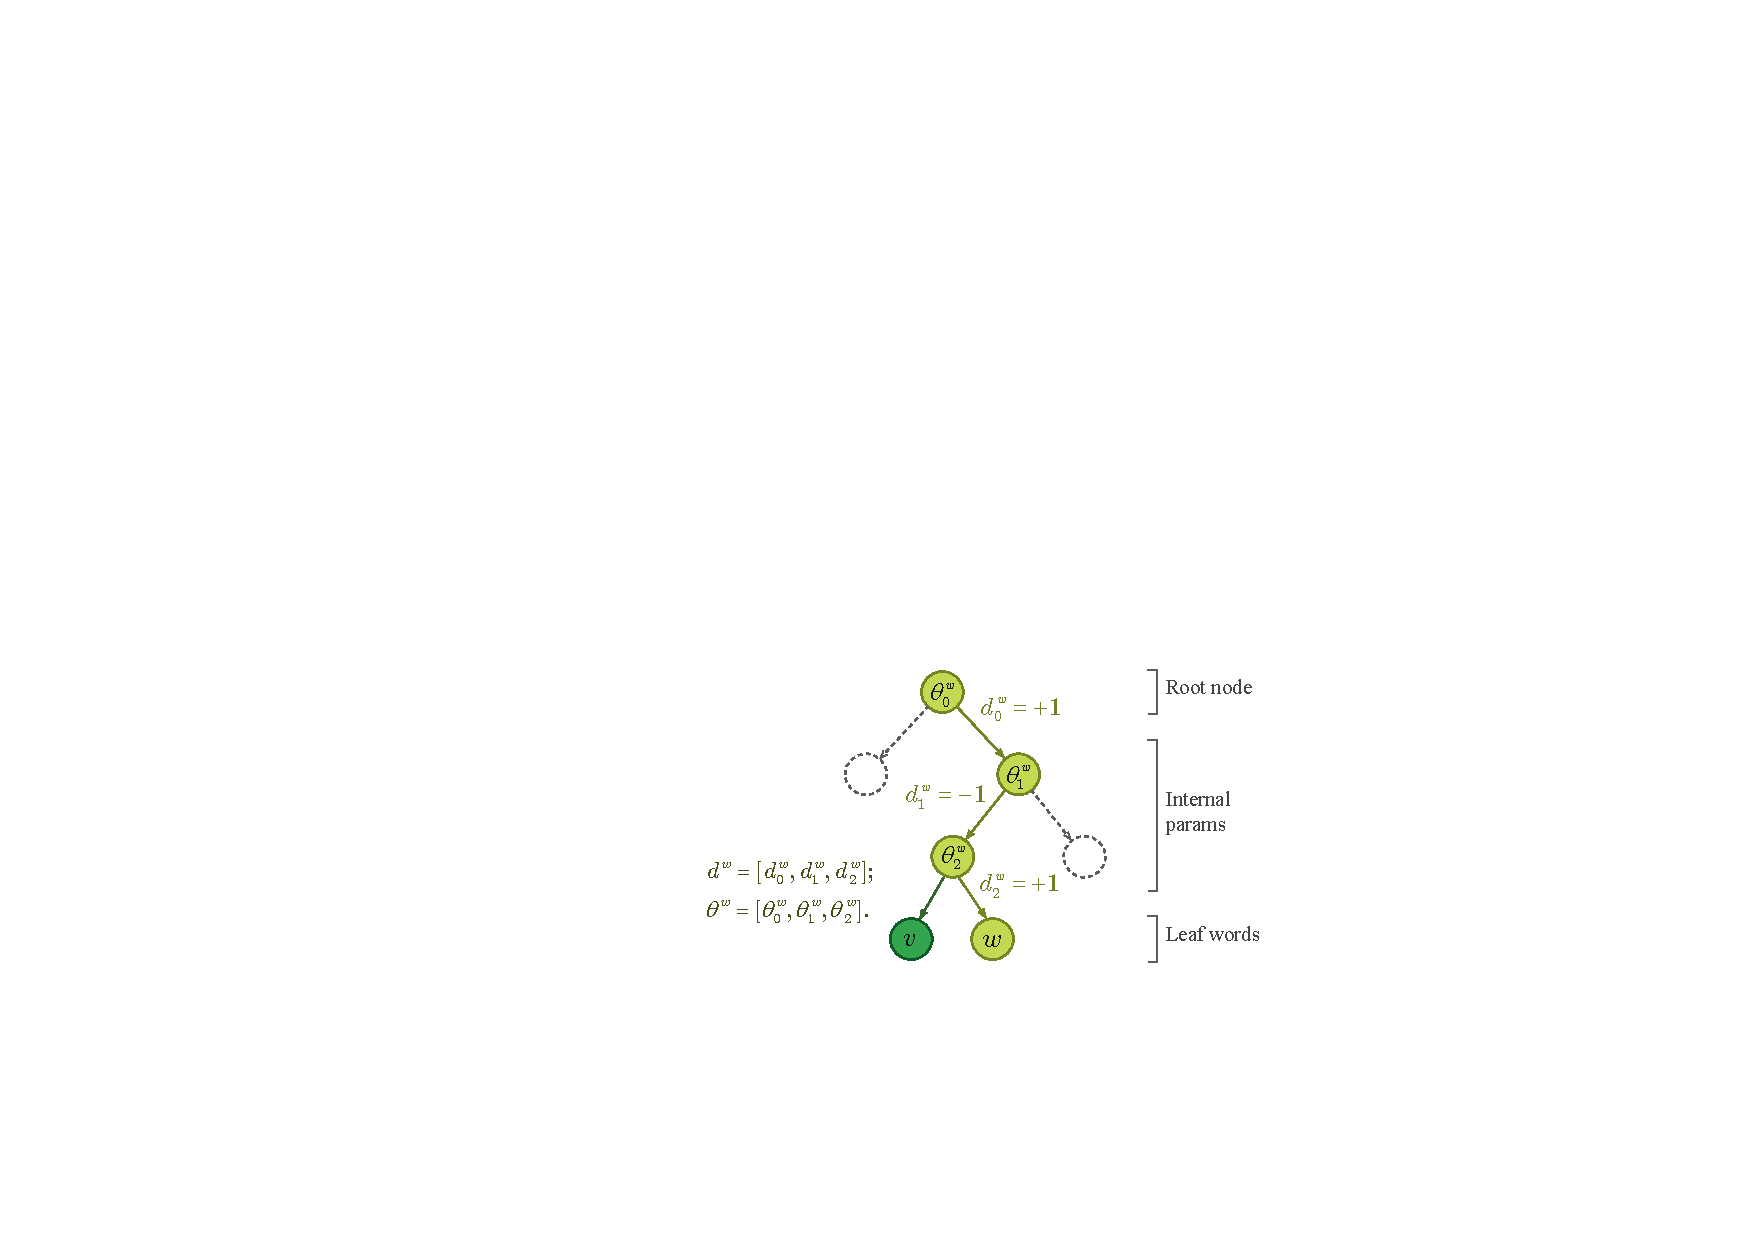
\includegraphics[width=0.7\linewidth]{thsm}}
      \caption{Tree-based Hierarchical Softmax. Internal nodes are parameterised by $\theta_i^w$, edges between nodes are parameterised by $d_i^w$, where $d^w$ is a vector and $\theta^w$ is a matrix.}
      \end{figure}
	probability for internal node $\theta_i^w$:
	\begin{equation}
    p(d^w_i=\pm 1|\theta_{i}^w,h) = \sigma({d_i^w}\theta_{i}^w h)
    \end{equation}
    log probability for word $w$:
    \begin{equation}
    \log p(w|h)=\log\prod_{i=0}^{l^w-1} p(d^w_i|\theta_{i}^w,h) = \sum_{i=0}^{l^w -1} \log\sigma(d_i^w \theta_{i}^w h)=\log\sigma({d^w}^\top \theta^w h)
    \end{equation}
    
    A major advantage: it avoids normalise the probability over the whole vocabulary, as the summarised probabilities of words in the tree equals to one.
\begin{equation}
\sum_{w\in \mathcal{V}}{p(w|h)}=\sum_{w \in \mathcal{V}}\sum_{i=0}^{l^w-1}{\sigma(d_i^w\theta_{i}^w h)}=1.
\end{equation}
    \end{block}
    \end{column}


    \begin{column}{.3\linewidth}
    

	\begin{block}{Why it is faster?}
Parallelised tree-based cost function:
    \begin{equation}
   \ell(\theta|h,w) =-\log\prod_{i=0}^{l^w -1} \sigma(d_i^w \theta_{i}^w h) = -\log \sigma({d^w}^\top \theta^w h)=  \zeta(- {d^w}^\top \theta^w h )
    \end{equation}
    Conventional cost function:
    \begin{equation}
    \ell'(\theta|h,w) =\sum_{i=0}^{l^w-1} \{(1-d'^w_i)\log (\sigma(\theta_{i}^w h))  + {d'^w_i}\log (1-\sigma (\theta_{i}^w h))\}
    \end{equation}
    \textbf{Two Main difference:}
	\begin{itemize}
	\item tHSM algorithm involves many tiny matrix multiplications, instead in p-tHSM we load all parameters $(d^w, \theta^w)$ directly as 1D vector and 2D matrix at the expense of runtime memory consumption and we consider the multiplications of this vector and giant matrix;
    \item A compact loss function of the model is deducted and the nodes' log-probability are calculated simultaneously which results in better time efficiency for p-tHSM model.
	\end{itemize}
      \end{block}
      \begin{block}{Experiment setups}
      \textbf{Dataset Statistics}: Number of tokens for train, valid and test, vocabulary size, and fraction of out-of-vocabulary rate.
      \begin{table}
      
        \setlength{\abovecaptionskip}{0pt}
        \setlength{\abovedisplayskip}{0pt}
        \centering
        \begin{tabular}{l|ccc|ccc|ccc}
        \toprule
        &\multicolumn{3}{c|}{PTB}&\multicolumn{3}{c|}{WikiText-2}&\multicolumn{3}{c}{WikiText-103}  \\
        &train& valid&test&train& valid&test&train & valid &test\\ \midrule
        Articles  & 2,000& 155& 155& 600& 60& 60& 28,475& 60 & 60\\
        Sents & 42,068   & 3,370  & 3,761 &36,718   & 3,760 & 4,358& 1,801,350   & 3,760 & 4,358 \\\midrule
        Vocab &\multicolumn{3}{c|}{10,000}&\multicolumn{3}{c|}{33,278} & \multicolumn{3}{c}{ 267,735}\\
        OOV &\multicolumn{3}{c|}{4.8\% }&\multicolumn{3}{c|}{2.6\% } & \multicolumn{3}{c}{0.4\%} \\
        \bottomrule
        \end{tabular}
       \end{table}
       
       % \vspace{2ex}
%       \textbf{Metrics}
%       \begin{itemize}
%    \item \textbf{Runtime benchmark}: efficiency, scalability, parameters size;
%    \item \textbf{Perplexity:} the degree of confusion when choosing the next utterance.
%    \end{itemize}
      \end{block}
      \begin{block}{Runtime benchmark}
      \begin{figure}
      \centering{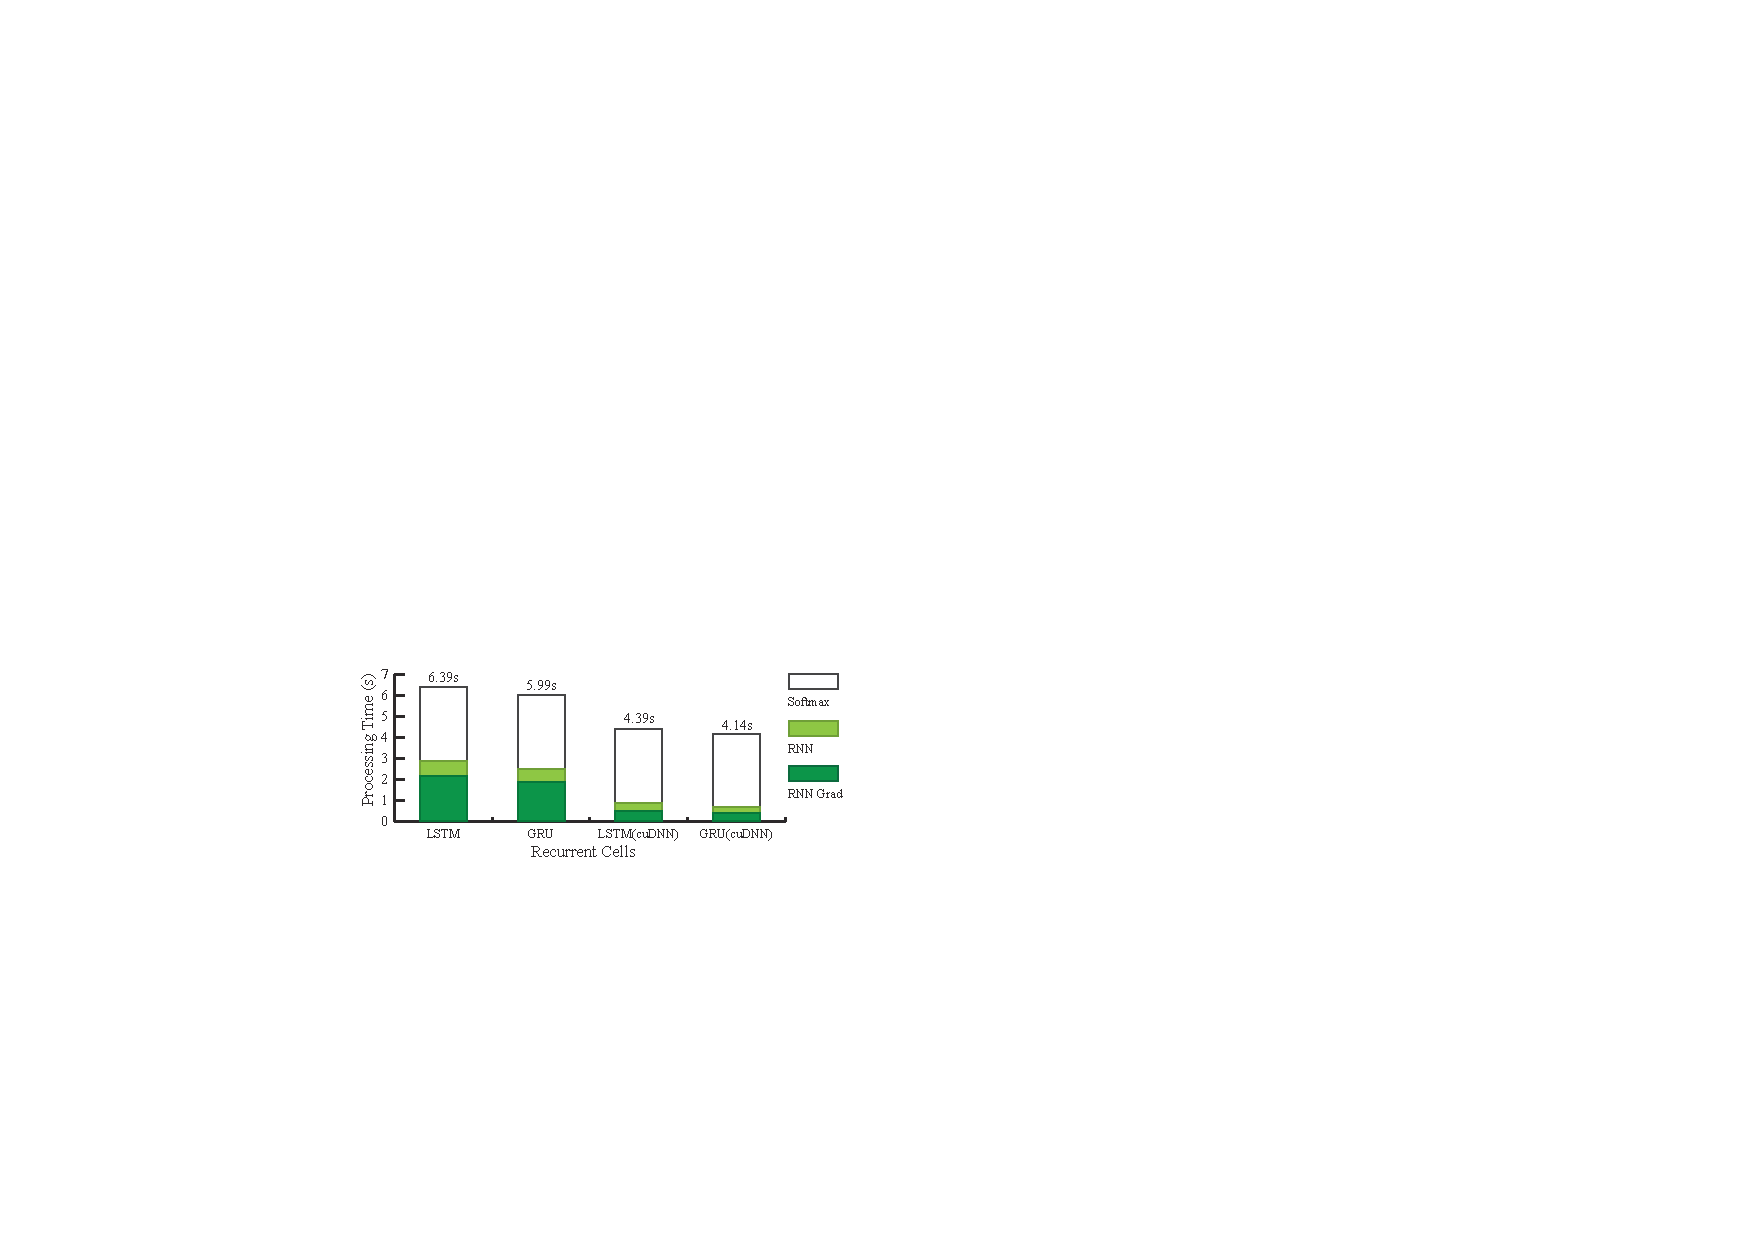
\includegraphics[width=0.65\linewidth]{rnn_timing}}
      %\caption{.}
      \setlength{\abovecaptionskip}{0pt}
      \setlength{\abovedisplayskip}{0pt}
      \setlength{\belowcaptionskip}{0pt}
      \setlength{\belowdisplayskip}{0pt}
      \end{figure}
      \textbf{Large Vocab Problem:} Calculation Time of three modules with different recurrent cells on Wikitext-103.
      \begin{figure}\small
      \centering{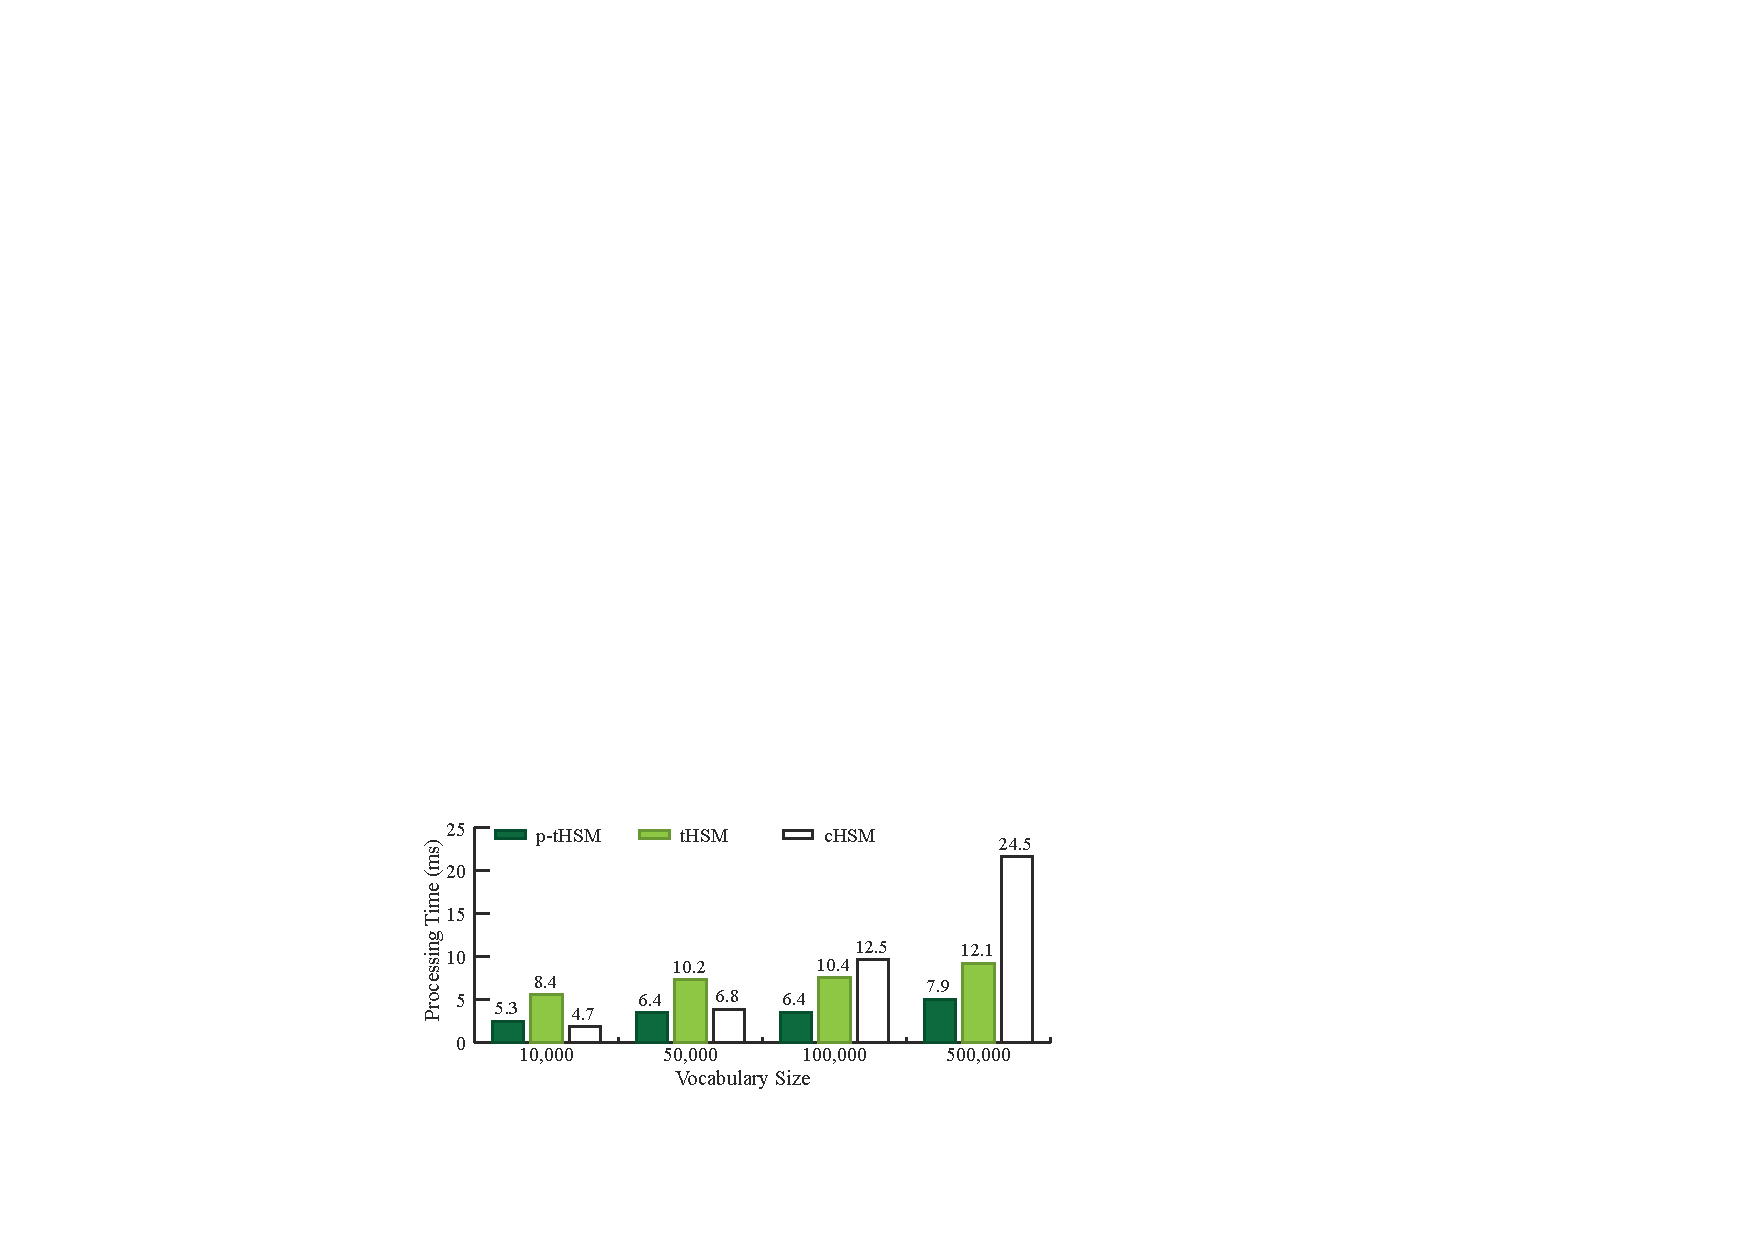
\includegraphics[width=0.65\linewidth]{all_time}}
      %\caption{ }
      \setlength{\abovecaptionskip}{0pt}
        \setlength{\abovedisplayskip}{0pt}
        \setlength{\belowcaptionskip}{0pt}
        \setlength{\belowdisplayskip}{0pt}
      \end{figure}
      \textbf{Scalability:}  cHSM, tHSM and p-tHSM algorithms with different vocabulary size.
      \end{block}
    \end{column}
    
    

    \begin{column}{.3\linewidth}
    
    
    \textbf{Speed Comparison:} Time and memory comparison on GPUs and CPUs with WikiText-103 dataset.
    \begin{table}
    \setlength{\abovecaptionskip}{0pt}
    \setlength{\abovedisplayskip}{0pt}
    \centering
    %\caption{\label{tab:time}}
    \begin{tabular}{lccccc}
    \toprule
    &Runtime &\multicolumn{2}{c}{Total (ms)} & \multicolumn{2}{c}{Forward (ms)}   \\
    \cmidrule(lr){3-4}  \cmidrule(lr){5-6}
	&memory &cpu&gpu &cpu&	gpu \\ \midrule
    Softmax & $\mathcal{|HV|}$ &510.4  &262.1&352.2& 62.9 \\
    cHSM    & $2\mathcal{|H|\sqrt{|V|}}$&506.5  &\textbf{40.6}&28.7&14.6 \\
    tHSM    &$\mathcal{|H|}$&1,004.0 &444.4 & 8.1&  5.6   \\
    p-tHSM  &$\mathcal{|H|\log{|V|}}$ &\textbf{383.5}&	86.4 &\textbf{7.0}&	\textbf{1.4} \\
    \bottomrule
    \end{tabular}
    \end{table}

      \begin{block}{Perplexity Results}

    \textbf{Word Clustering Strategy Analysis}: apply different clustering methods to initialise the distribution of words over the tree.
    \begin{table}
   
    \setlength{\abovecaptionskip}{0pt}
    \setlength{\abovedisplayskip}{0pt}
  \centering
  %\caption{Perplexity of p-tHSM method with various hierarchical clustering algorithms on PTB Dataset.\label{table:clustering}}
  \begin{tabular}{lcc} \toprule
  Methods   & Valid & Test   \\ \midrule
  Random Shuffle &199.62 &  189.37\\
  Alphabetical Order  & 154.02 & 149.12       \\
  Huffman Clustering   & 134.33 & 129.34      \\
  Brown Clustering  & \textbf{133.12} & \textbf{128.78}\\
\bottomrule
  \end{tabular}
\end{table}

\vspace{3ex}
\textbf{All Experiments Benchmark:} Perplexity benchmark on validation and testing dataset with PTB, WikiText-2 and WikiText-103 corpus.
\begin{table}
\setlength{\abovecaptionskip}{0pt}
\setlength{\abovedisplayskip}{0pt}
  \centering
  %\caption{Perplexity benchmark on validation and testing dataset with PTB, WikiText-2 and WikiText-103 corpus.}\label{tab:summary}
\begin{tabular}{lcccccc}
  \toprule
  & \multicolumn{2}{c}{PTB} & \multicolumn{2}{c}{WikiText-2} & \multicolumn{2}{c}{WikiText-103} \\
  \cmidrule(lr){2-3} \cmidrule(lr){4-5} \cmidrule(lr){6-7}
  & Valid & Test& Valid & Test  & Valid & Test \\ \midrule
  GRU + Softmax                                             &\textbf{131.59}&\textbf{125.10} &\textbf{169.07}&\textbf{160.45}&170.19&171.02\\
  GRU + NCE             &139,79&137.35 &210.19&189.15&194.78&195.01\\
  GRU + Blackout          &137.68&135.49 &201.51&185.31&192.11&193.76\\
  GRU + cHSM                  &133.17&125.05 &179.64&169.09&171.81&166.74\\  \midrule
  GRU + p-tHSM + Huffman &134.33&129.34 &218.42&216.05& 165.70&166.11\\
GRU + p-tHSM + Brown &133.12&128.78       &186.23&189.58 &\textbf{164.15}& \textbf{161.55} \\
  \bottomrule
\end{tabular}
\end{table}
      \end{block}

      \begin{block}{Our Contributions}
	\begin{itemize}
	\item We propose a parallelised mathematical model for modeling vanilla hierarchical softmax algorithm, making it compatible with GPUs;
    \item Aiming at improving its stability, we employ several n-gram based and semantic clustering algorithms to initialise the word hierarchy before the training stage;
    \item We conducted empirical analysis and comparisons on the standard PTB, WikiText-2 and WikiText-103 datasets with other traditional optimisation methods to assess its efficiency and accuracy on GPUs and CPUs.
	\end{itemize}
      \end{block}
    \end{column}
  \end{columns}
\end{frame}
\end{document}

